\chapter{Introduction}
\label{cha:chapter1}
In recent years, machine learning (ML) has been increasingly involved in almost every aspect of our life, for example, recommendation systems on e-commerce sites, medical diagnosis, or self-driving cars. This development can not be achieved without intelligent algorithms behind. A particular type of ML algorithms, called neural networks (NNs), have been gradually used to power such systems.  This is because NNs have directly benefitted from the vast amount of data available and more efficient computation resources developed, giving a much better performance as compared to other ML algorithms. As a result, intelligent systems we use nowadays frequently rely on them.

In short, NNs are algorithms inspired by how the human brain works. One of their advantages is that they can learn patterns from data efficiently. NNs comprise of simple units, called neurons, arranged in layers working together to transform input to the desired output. When the network is comprised of many layers, it is often referred to as \textit{deep learning}. Connections between neurons define this transformation. These connections are learned from the training data without being explicitly defined. 

Because the transformation is typically in high dimensional space and built to a specific problem, it is not apparent to us how the trained NN utilizes input and makes a prediction.  This lack of understanding raises concerns and questions to the machine learning community and consumers. One primary concern is about trust, in particular, how we can ensure that NNs will work as we expect. Secondly, not having this insight results in considerable amount of trials and errors when it comes to adjusting configurations of NNs to achieve expected performance.

Researchers have proposed several methods to understand better or explain how NNs transform input to output. In particular, \citet{SimonyanDeepConvolutionalNetworks2013}  proposed a pioneer work in understanding predictions of NNs through the \textit{activation maximization} approach and a method relying on partial derivatives which we refer to as \textit{sensitivity analysis} (SA). \citet{SpringenbergStrivingSimplicityAll2015a} suggested a modified version of SA, called \textit{guided backprop} (GB), for ReLU-type NNs. In the results, GB produces more informative explanations than SA. \citet{SmilkovSmoothGradremovingnoise2017}  proposed \textit{SmoothGrad} technique to improve quality of SA explanations. 

\cite{BachPixelWiseExplanationsNonLinear2015} proposed an alternative approach, called \textit{Layer-wise Relevance Propagation} (LRP). The method utilizes architecture of the NN itself to create explanations, instead of relying on derivatives as in SA and GB. For ReLU-type networks, \citet{MontavonExplainingnonlinearclassification2017} derived  the \textit{deep Taylor decomposition} (DTD) technique for explaining their non-linear decisions. They showed that DTD is a special case of LRP. \citet{SundararajanAxiomaticAttributionDeep2017a} proposed the \textit{integrated gradients} method combining gradient and decomposition techniques. \citet{RibeiroWhyShouldTrust2016} developed \textit{Local Interpretable Model-Agnostic Explanations} (LIME) framework that can explain predictions from a wider set of models. \citet{OlahBuildingBlocksInterpretability2018} suggested ideas for visualizing explanations from multiple domains. 

These works have primarily focused on standard NNs or feedforward architectures. However, there is still only a limited number of contributions in explaining predictions from recurrent neural networks (RNNs). RNNs are essential algorithms in domains that pprocess sequential data, such as machine translation and natural language processing (NLP). To the best of our knowledge, the closest works in this direction are from 1) \citet{KarpathyVisualizingUnderstandingRecurrent2015} that  interpreted activations of LSTM \citep{HochreiterLongshorttermmemory1997} cells for a certain task and 2) \citet{ArrasExplainingRecurrentNeural2017} that applied LRP to a LSTM network trained to perform a sentiment analysis task. Therefore, a study of these explanation techniques for RNNs needs to be explored. This understanding study will enable us to gain insight how RNNs internally work and hopefully it will lead us to develop more explainable RNN architectures.


%In fact, state-of-the-art of these applications today mostly rely on RNN. However, the question of how neural networks, including RNN, derive their predictions is still unclear to us. This causes resistance in the adoptation and development of the technology itself. 

%
%
%However, there is still only few work in the direction of explaining predictions from RNN. 
%
%
% Although these work has demonstrated promising results on neural networks, more specifically feed-forward architectures, there is still only a few applications of these methods to recurrent architecture. These recurrent neural networks are considerably important and have been powering almost machine learning systems processing sequential data, such as machine translation and natural language understanding. Therefore, applications of these explanation techniques to recurrent neural networks need to be explored. This results will also enable us to propose adjustments to recurrent architectures such that they are more explainable.


\section{Objective \& Scope}
This thesis aims to explain RNN predictions. More precisely, the goal of this thesis is to study how the structure of RNNs affects the quality of explanations produced by various explanation techniques. In particular, we are interested in applying explanation techniques that were developed for feedforward architectures, such as sensitivity analysis, guided backprop, layer-wise relevance propagation and deep Taylor decomposition to the RNN setting. 

Our study is based on artificial classification problems that are specially constructed such that knowledge of ground truth explanations is available to us. As a result, we can perform qualitative and quantitative measurements accordingly.


We hypothesize that RNNs with more layers are more explainable than ones with fewer layers. We conduct extensive experiments on various configurations to verify our proposition. We also propose an adjustment to LSTM. This adjustment allows us to apply the explanation techniques mentioned above to the LSTM architecture.

Lastly, because we consider the harder case where data arrives sequentially and not all at once like convolutional neural networks (CNNs), classification accuracy is limited by this more challenging setting. Therefore, we do not seek to train models to achieve the state-of-the-art performance. We instead train them to reach a certain level of accuracy. We assume that models operating at this level are good enough and produce comparable explanations. 
%
%as the primary goal is to study explainability of RNNs, it is worth mentioning that we do not seek to train models to achieve the state-of-the-art performance. We instead train them to reach a certain level of accuracy. We assume that models operating at this level are good enough and produce comparable explanations. In fact, the classification problems we are considering are harder cases because data arrives sequentially and not all at once like convolutional neural networks (CNNs). Therefore, classification accuracy is limited by this more challenging setting. 


%assumption relu? ... 
%
%not care performance much ..
%
%our hypothesis ... 
%
%artificial problems ... 


%\section{Dataset}
%Our study is based on MNIST\citep{LeCunMNISThandwrittendigit2010} and FashionMNIST\citep{XiaoFashionMNISTNovelImage2017}. Following is a brief introduction of them.
%
%\subsection{MNIST}
%
%\begin{figure}[!hbt]
%	\centering
%	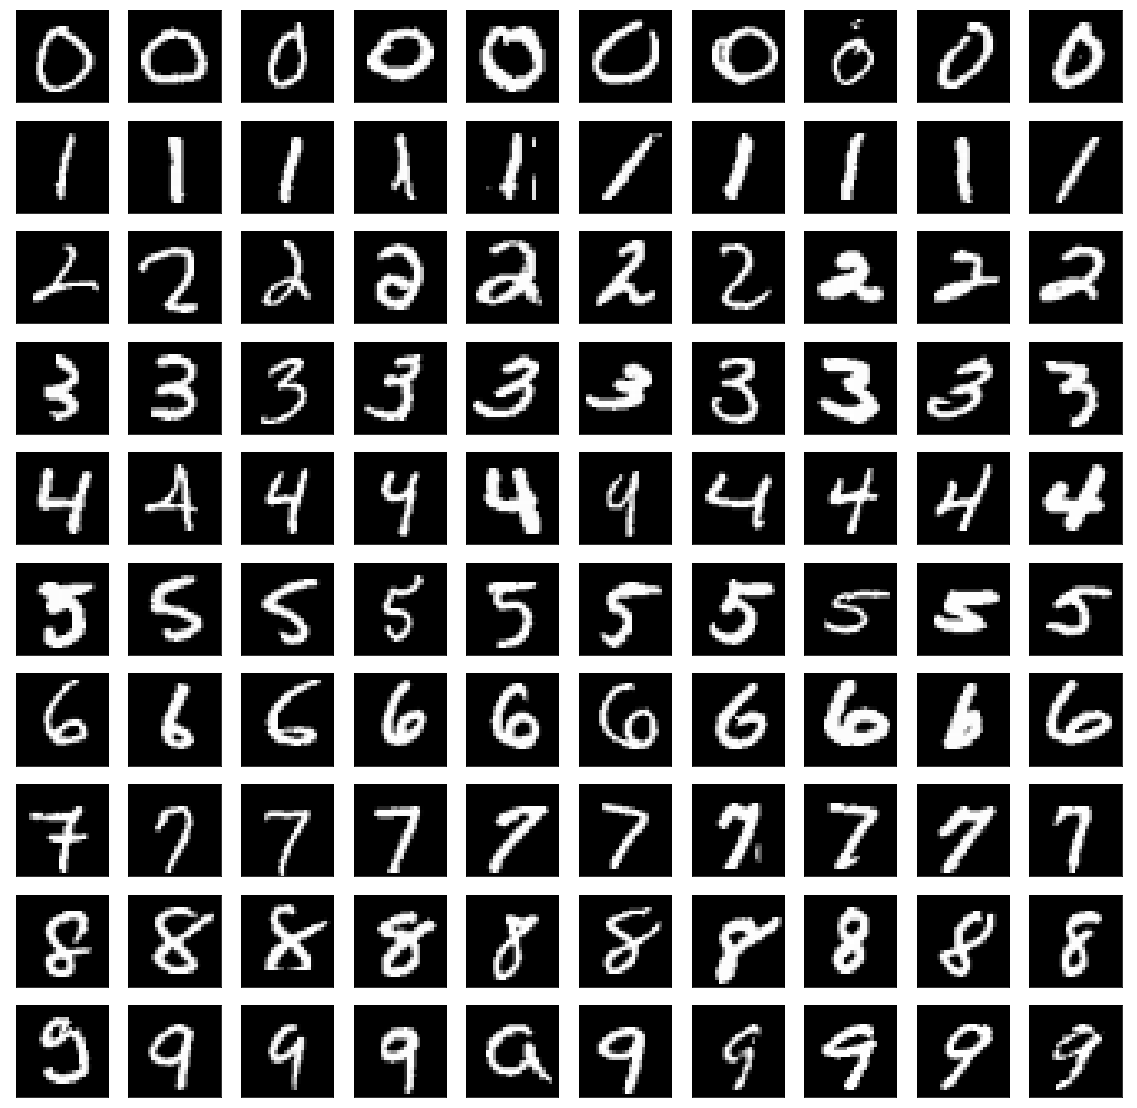
\includegraphics[width=0.6\textwidth]{mnist}
%	\caption{MNIST dataset.}
%	\label{fig:mnist_samples}
%\end{figure}
%
%MNIST is one of the most popular dataset that machine learning partitioners use to benchmark machine learning algorithms. The dataset consists of 60,000 training and 10,000 testing samples. Each sample is a grayscale 28x28 image. As shown in \addfigure{\ref{fig:mnist_samples}}, MNIST has 10 categories corresponding to a digit between 0 and 9.
%
%
%State-of-the-art algorithms can classify MNIST with accuracy higher than 99\%, while classical ones, such as SVC or RandomForest, are able to achieve around 97\%\citep{XiaoFashionMNISTNovelImage2017}.
%
%
%\subsection{FashionMNIST}
%
%FashionMNIST is a dataset \todo{ rephrase : whose authors aim to it to be a replacement of MNIST, especially in  benchmarking machine learning algorithms}.  According to \citep{XiaoFashionMNISTNovelImage2017},  FashionMNIST is more representative to modern computer vision tasks. It contains images of fashion products from 10 categories and compatible  to MNIST in every aspects, such as the size of training and testing set, image dimension and data format, hence one can easily  apply existing algorithms that work with MNIST to Fashion-MNIST without any change. \addfigure{\ref{fig:fashion_mnist_samples}} shows FashionMNIST samples.
%
%\begin{figure}[!hbt]
%\centering
%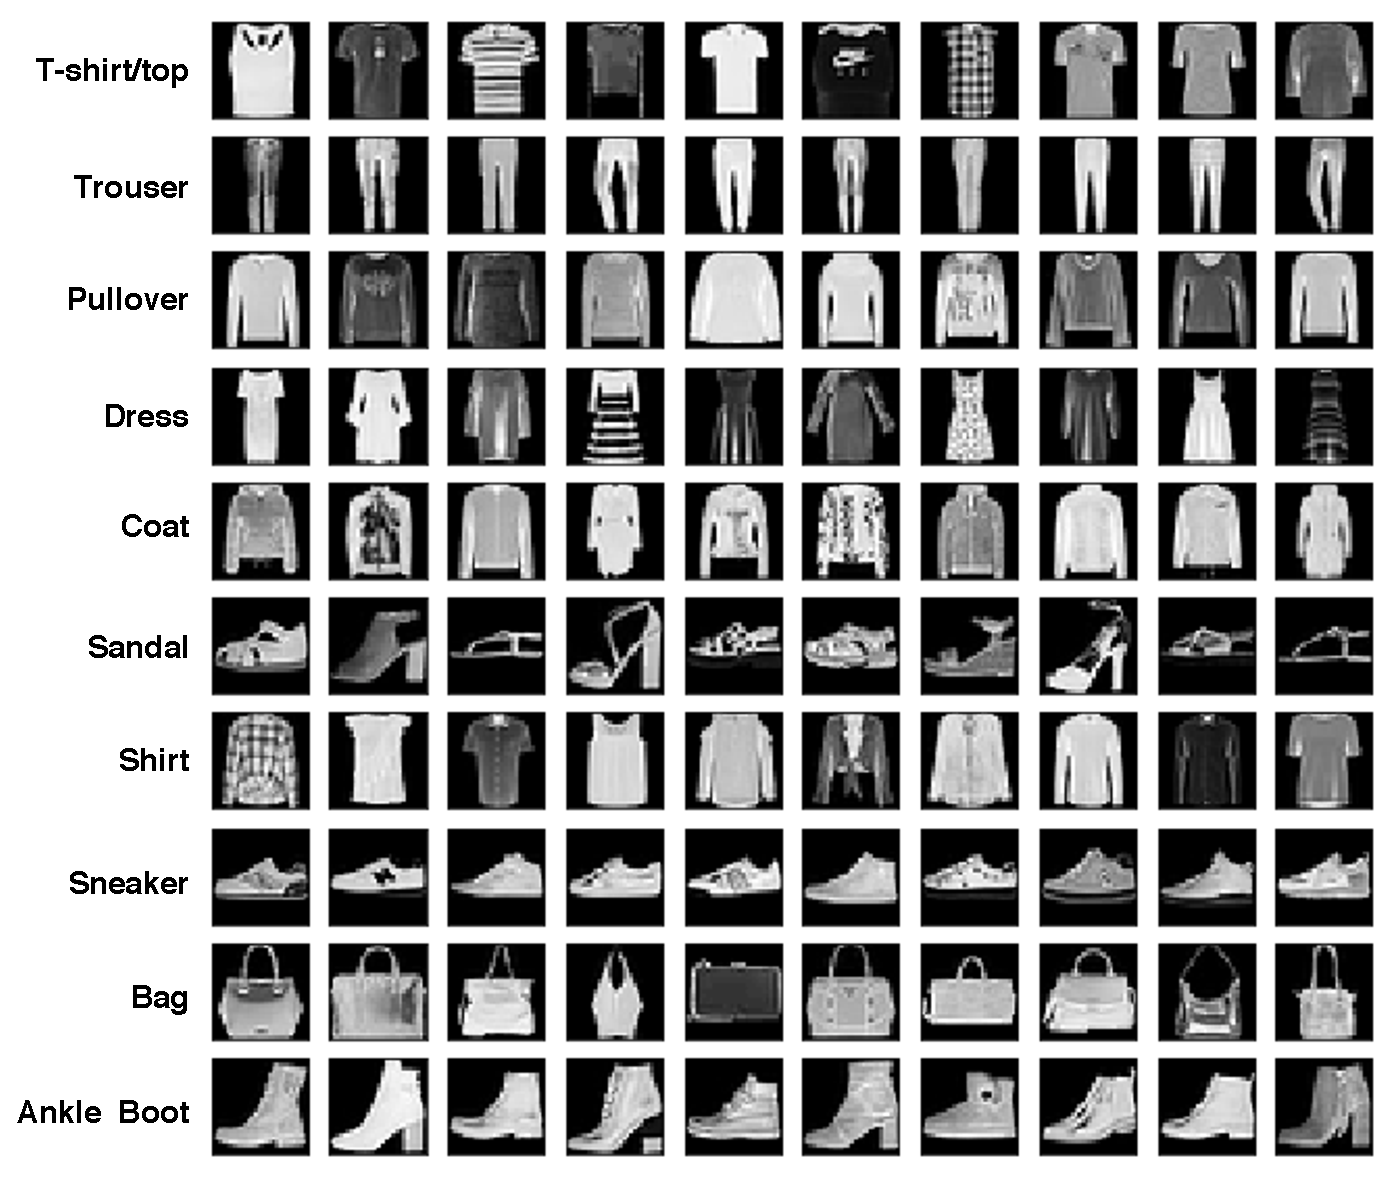
\includegraphics[width=0.65\textwidth]{sketch/fmnist_samples}
%\caption{FashionMNIST dataset.}
%\label{fig:fashion_mnist_samples}
%\end{figure}
%
%\citet{XiaoFashionMNISTNovelImage2017} also reports benchmarking results of classical machine learning algorithms on Fashion-MNIST. On average, they achieve accuracy between 85\% to 89\%. According to Fashion-MNIST's page\footnote{https://github.com/zalandoresearch/fashion-mnist}, state-of-the-art result has 97\% accuracy using Wide Residual Network(WRN)\citep{ZagoruykoWideResidualNetworks2016} and standard data preprocessing and augmentation.

%\section{Terminology}
%\todo{terminology}

\clearpage

\section{Outline}
The thesis is organized as follows:
\begin{itemize}
%	\item \textbf{Chapter \ref{cha:chapter2}} provides a brief literature survey and related work in the direction towards explaining neural networks.
	\item \textbf{Chapter \ref{cha:chapter3}} summarizes relevant topics in  neural networks and explanation techniques that are focused in the thesis.
	\item \textbf{Chapter \ref{cha:chapter4}} is devoted to experimental results.
	\item \textbf{Chapter \ref{cha:chapter5}} concludes the results and discusses challenges as well as future work.
\end{itemize}

%
%This chapter should have about 4-8 pages and at least one image, describing your topic and your concept. Usually the introduction chapter is separated into subsections like 'motivation', 'objective', 'scope' and 'outline'.
%
%\section{Motivation\label{sec:moti}}
%
%Start describing the situation as it is today or as it has been during the last years. 'Over the last few years there has been a tendency... In recent years...'. The introduction should make people aware of the problem that you are trying to solve with your concept, respectively implementation. Don't start with 'In my thesis I will implement X'.
%
%\section{Objective\label{sec:objective}}
%
%What kind of problem do you adress? Which issues do you try to solve? What solution do you propose? What is your goal?
%'This thesis describes an approach to combining X and Y... The aim of this work is to...'
%
%\section{Scope\label{sec:scope}}
%
%Here you should describe what you will do and also what you will not do. Explain a little more specific than in the objective section. 'I will implement X on the platforms Y and Z based on technology A and B.'
%
%Conclude this subsection with an image describing 'the big picture'. How does your solution fit into a larger environment? You may also add another image with the overall structure of your component.
%
%'Figure \ref{fig:intro} shows Component X as part of ...' 
%\\
%\begin{figure}[htb]
%  \centering
%  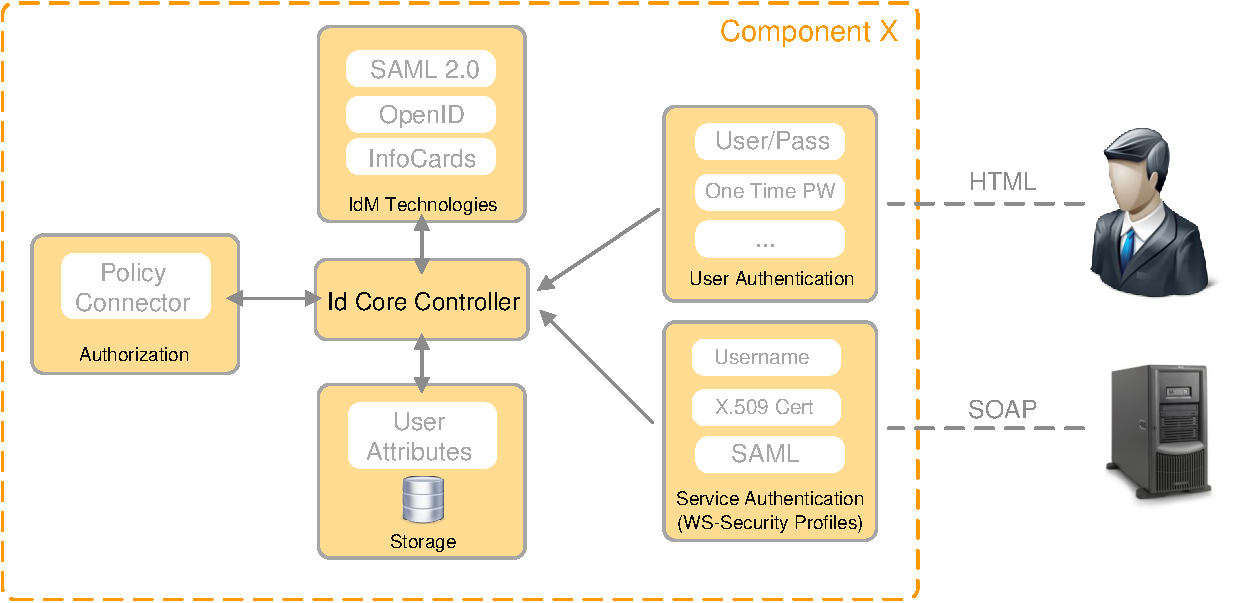
\includegraphics[width=9cm]{intro_example.pdf}\\
%  \caption{Component X}\label{fig:intro}
%\end{figure}
%
%\section{Outline\label{sec:outline}}
%
%The 'structure' or 'outline' section gives a brief introduction into the main chapters of your work. Write 2-5 lines about each chapter. Usually diploma thesis are separated into 6-8 main chapters. 
%\\
%\\
%\noindent This example thesis is separated into 7 chapters.
%\\
%\\
%\textbf{Chapter \ref{cha:chapter2}}  Neural Network and Explainability foudation
%%is usually termed 'Related Work', 'State of the Art' or 'Fundamentals'. Here you will describe relevant technologies and standards related to your topic. What did other scientists propose regarding your topic? This chapter makes about 20-30 percent of the complete thesis.
%\\
%\\
%\textbf{Chapter \ref{cha:chapter3}} Architecture
%%analyzes the requirements for your component. This chapter will have 5-10 pages.
%\\
%\\
%\textbf{Chapter \ref{cha:chapter4}} Experiments
%%Ais usually termed 'Concept', 'Design' or 'Model'. Here you describe your approach, give a high-level description to the architectural structure and to the single components that your solution consists of. Use structured images and UML diagrams for explanation. This chapter will have a volume of 20-30 percent of your thesis.
%\\
%\\
%\textbf{Chapter \ref{cha:chapter5}} Conclusion and future work
%%describes the implementation part of your work. Don't explain every code detail but emphasize important aspects of your implementation. This chapter will have a volume of 15-20 percent of your thesis.
%%\\
%\\
%%\textbf{Chapter \ref{cha:chapter6}} is usually termed 'Evaluation' or 'Validation'. How did you test it? In which environment? How does it scale? Measurements, tests, screenshots. This chapter will have a volume of 10-15 percent of your thesis.
%%\\
%%\\
%%\textbf{Chapter \ref{cha:chapter7}} summarizes the thesis, describes the problems that occurred and gives an outlook about future work. Should have about 4-6 pages.